\section{Frontend - Webapplikation als REST-Client}
\subsection{Überblick}
Das \Gls{backend} muss mit dem \Gls{frontend} verbunden werden.Es gibt unterschiedliche Möglichkeiten dies zu realisieren. Beim Realisieren, muss darauf geachtet werden, dass eine Struktur vorhanden ist. Es werden 2 verschiedene \Gls{designpattern} angeschaut und verglichen. Umgesetzt wird dann ein \Gls{designpattern} mithilfe von \Gls{js}. Hier kann ein \Gls{jsframework} zum Einsatz kommen. Dazu werden hier verschiedene \Gls{jsframework}s angeschaut und verglichen. Für die Verarbeitung der Daten ist es wichtig Datenformate festzulegen. Die Aufbereitung der Elemente fürs \Gls{frontend} mit den Daten des \Gls{backend}s wird ebenfalls angeschaut.
\subsection{Entwurfsmuster}
Dieser Teil des Projektes wird in Verwendung eines \Gls{designpattern}s umgesetzt. Zwei \Gls{mv*} \Gls{designpattern}s werden hierbei in Betrachtung gezogen. Zum einen \Gls{mvvm} und zum anderen \Gls{mvc}. Es kommen diese zwei Entwurfsmuster in Frage, da \Gls{mvc} in sehr bekanntes \Gls{designpattern} ist und MVVM eine neuere Variante von \Gls{mvc} ist.
\subsubsection{MVC}
\Gls{mvc} ist ein \Gls{designpattern} mit dem eine Software in die drei Teile (Model, View und Controller) geteilt wird.\\
Das Model beinhaltet alle Daten der Software und auch alle Funktionen, die mit den Daten interagieren oder mit ihnen rechnen.\\
Die View ist der Teil der Software, die Benutzer*innen sehen und mit denen sie interagieren. Dieser Teil der Software beinhaltet keine wichtigen Daten oder Funktionen, welche Daten bearbeiten. Sie hört nur auf Benutzereingaben und zeigt die bereitgestellten Daten an.\\
Der Controller ist der Teil der Software, der Model und View verbindet. In dem Controller wird auf die Benutzereingaben reagiert und die richtigen Funktionen aus dem Model aufgerufen.\cite{mvc}
\begin{figure}[H]
	\centering
	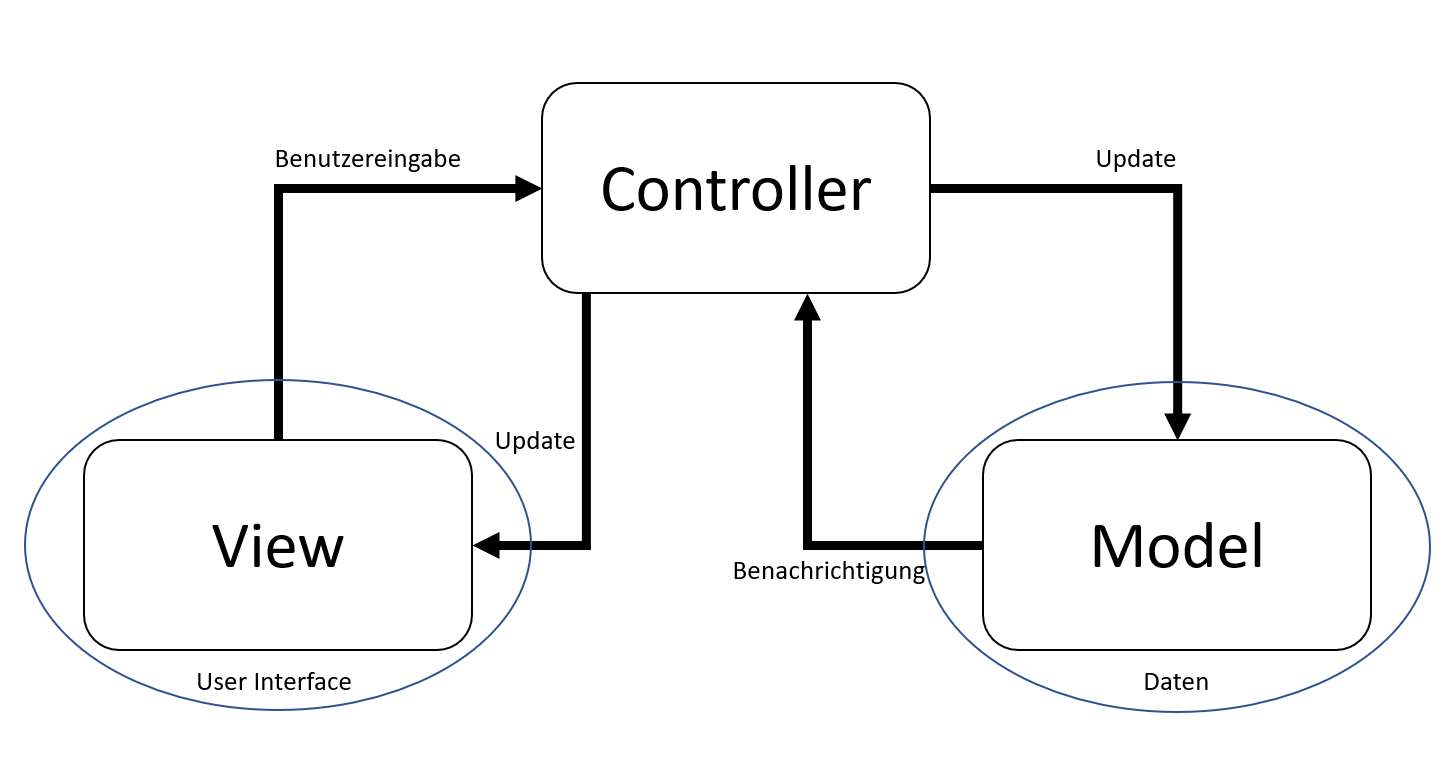
\includegraphics[width=0.8\linewidth]{images/mvc}
	\caption[Übersicht des MVC-Patterns]{Übersicht über die Komponenten des MVC-Patterns und ihre Zusammenhänge}
	\label{fig:mvc}
\end{figure}
\subsubsection{MVVM}
\Gls{mvvm} oder auch MVVC ist ein \Gls{designpattern} mit dem eine Software in drei Teile geteilt wird. Jedoch wird bei \Gls{mvvm} die Software in Model, View und ViewModel aufgeteilt.\\
Das Model beinhaltet wie im konventionellen \Gls{mvc}-Pattern alle wichtigen Daten und Funktionen.\\
Die View ist wie beim \Gls{mvc}-Pattern der Teil der Software, mit der Benutzer*innen interagieren.\\
Das ViewModel ist ein Bindeglied zwischen Model und View. Dabei stellt es der View offen Funktionen zur Verfügung. Diese können auch Daten verändern bzw. mit Daten rechnen. Das Model kann über das ViewModel auch mit der View direkt interagieren.\\
\Gls{mvvm} sieht nicht vor, dass ein Controller verwendet wird. Diese Funktion übernimmt zu einem gewissen Teil das ViewModel bzw. auch die View und das Model.\cite{mvvm_vue}
\begin{figure}[H]
	\centering
	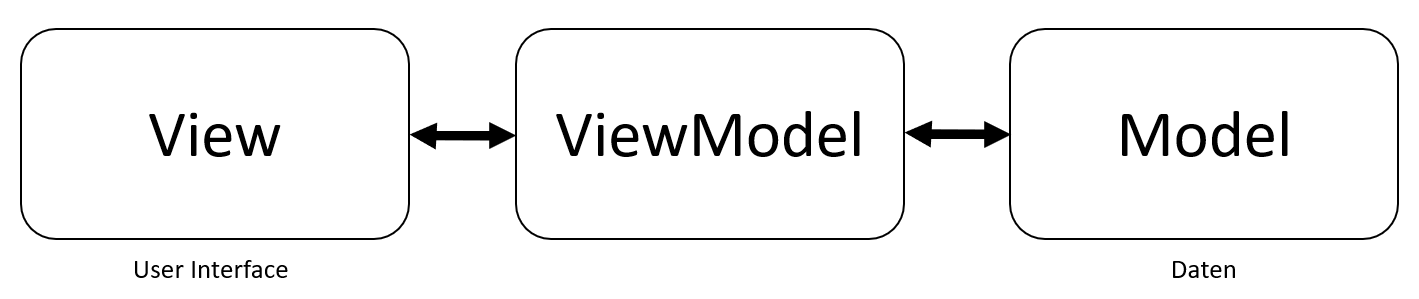
\includegraphics[width=0.8\linewidth]{images/mvvm}
	\caption[Übersicht des MVVM-Patterns]{Übersicht über die Komponenten des MVVM-Patterns und ihre Zusammenhänge}
	\label{fig:mvvm}
\end{figure}
\newpage
\subsubsection{Vergleich}
Diese zwei \Gls{designpattern} sind zwar sehr ähnlich, jedoch gibt es Unterschiede zwischen ihnen.\\\\
\Gls{mvc} ist ein Entwurfsmuster, welches auf einem niedrigen Level überall im Einsatz ist wie z.B.: bei Tastatureingaben. Dieses \Gls{designpattern} ist zwar schon lange Verfügbar, jedoch kann es bei Webapplikationen zu Problemen führen.\\
Bei der Entwicklung einer Webapplikation ist es nicht simpel, das Model von dem Controller zu trennen.\\
\Gls{mvvm} auf der anderen Seite, zielt explizit auf HTML5 ab.\cite{mvvm_vue} Somit ist es bei Webbasierten Applikationen zu bevorzugen.
\subsection{Datenformate}
\newpage
\subsection{Umsetzungsmöglichkeiten}
Dieser Teil des Projekts wird mittels \Gls{js} umgesetzt. Hierbei kommen unterschiedliche \Gls{jsframework} in Frage. Hier werden die verbreitesten \Gls{jsframework}s vorgestellt und dann verglichen.
\subsubsection{Vue}
\gls{vue} ist ein progressives \Gls{jsframework}. Dies bedeutet, dass Vue in bereits bestehende Webseiten bzw. Webbasierte Software implementiert werden kann.\\
\Gls{vue} kann aber auch von Anfang an verwendet werden, wobei man hier mit den Bibliotheken von \Gls{vue} skalieren kann. \Gls{vue} kann Teile einer Website in Komponenten aufteilen, um diese öfters zu verwenden, falls dies notwendig ist. Jeder dieser Komponenten hat sein eigenes \Gls{html}, \Gls{css} und \Gls{js} File, was gebraucht wird, um diese Komponente zu rendern.\cite{vuedoc}\\
Um einzelnen Elementen \Gls{vue}-Funktionalität zu geben kann auf diese Elemente folgender Code angewendet werden:
\begin{code}{html}
	<!DOCTYPE html>
	<html lang="de">
		<head>
			<meta charset="UTF-8">
			<meta name="viewport" content="width=device-width, initial-scale=1.0">
			<title>Kurzes VueJS-Beispiel</title>
		</head>
		<body>
			<h1>Überschrift</h1>
			<div id="app">
				<p> {{ text }} </p>
			</div>
			<script src="https://unpkg.com/vue"></script>
			<script>
				const app = new Vue({
					el: '#app',
					data: {
						text: 'Hier steht Text!'
					}
				})
			</script>
		</body>
	</html>
\end{code}
\cite{vuedoc}
\newpage
\subsubsection{React}
\Gls{react} ist eine \Gls{js}-Bibliothek, mit der man Benutzeroberflächen entwickeln kann. \Gls{react} hat wie \Gls{vue} Komponenten. Dies bedeutet, dass man einzelne Elemente öfters verwenden kann, falls man dies benötigt.\\
\Gls{react} ist von Facebook entwickelt worden und wurde 2013 als \Gls{opensource}-Lösung veröffentlicht.\cite{reactdoc}\\
Folgender Code beschreibt eine Beispiel-React Website:
\begin{code}{html}
	<!DOCTYPE html>
	<html lang="de">
		<head>
			<meta charset="UTF-8">
			<meta name="viewport" content="width=device-width, initial-scale=1.0">
			<title>Kurzes React-Beispiel</title>
		</head>
		<body>
			<h1>Überschrift</h1>
			<div id="likebuttoncontainer"></div>
			
			<!-- Load React. -->
			<!-- Note: when deploying, replace "development.js" with "production.min.js". -->
			<script src="https://unpkg.com/react@17/umd/react.development.js" crossorigin></script>  <script src="https://unpkg.com/react-dom@17/umd/react-dom.development.js" crossorigin></script>
			<!-- Load our React component. -->
			<script src="likebutton.js"></script>
		</body>
	</html>
\end{code}
\cite{reactdoc}
In der letzten Zeile des body-tags, wird auf ein "likebutton.js" referenziert. Dies ist eine Komponente und muss noch erstellt werden:
\begin{code}{js}
	'use strict';
	
	const e = React.createElement;
	
	class LikeButton extends React.Component {
		constructor(props) {
			super(props);
			this.state = { liked: false };
		}
		
		render() {
			if (this.state.liked) {
				return 'You liked this.';
			}
			
			return e(
			'button',
			{ onClick: () => this.setState({ liked: true }) },
			'Like'
			);
		}
	}
	
	const domContainer = document.querySelector('#likebuttoncontainer');
	ReactDOM.render(e(LikeButton), domContainer);
\end{code}
\cite{reactdoc}
\subsubsection{Angular}
\subsubsection{Ohne Framework}
\subsubsection{Vergleich}
\subsection{Aufbereitung der Daten}
\subsection{Fragestellung}